\chapter{Support Vector Machines}
\label{chap:svm}
Support Vector Machines (\glspl{svm}) are supervised machine learning models that are used in their canonical form for linear (binary\footnote{Multiclass classification can be achieved via techniques such as \textit{one-against-all} or \textit{one-against-one}~\cite{svmmulticlass}.}) classification and regression, as well as for anomaly detection (\eg{}, Ref.~\cite{svm}).
In its simplest form (hard margin), the training objective of an \gls{svm} for a binary classification task is the parametrization of a hyperplane with normal vector $\vec{w}$ and offset $b$ (\ie{}, $\vec{y}$ in plane $\Leftrightarrow$ $\vec{w} \cdot \vec{y} + b = 0$) such that $|\vec w|_2$ becomes minimal and all instances of different classes are separated by the hyperplane, \ie{},
$$t_i \left( \vec{w} \cdot \vec{x}^{\,(i)} + b \right) \ge 1 \; \forall \, i,$$
where $x^{\,(i)} \in \mathbb{R}^n$ is the feature vector of the $i$-th instance and $t_i$ is given by the respective label vector $y_i \in \mathbb{R}^n$,
\begin{equation*}
t_i := \begin{cases}
    +1 & \text{if } y_i \sim \text{signal}, \\
    -1 & \text{if } y_i \sim \text{background}. \\
\end{cases}
\end{equation*}
Instances with the minimal distance $t_i \left( \vec{w} \cdot \vec{x}^{\,(i)} + b \right) = 1$ are considered to lie on the \textit{margin} and are thus referred to as the \textit{supporting vectors} of the classifier (hence the name).
Obviously, the hard margin problem is only solvable for linearly separable data.
By introducing slack variables $\zeta_i \ge 0$ for each instance $i$, this constraint is relaxed
\begin{equation}
    \label{eq:apdx_svm}
    \underset{\vec w, b, \vec \zeta}{\operatorname{argmin}} \, \frac{1}{2} |\vec{w}|_2^2 + C |\vec \zeta|_1
    \quad \text{subject to }
    t_i \left( \vec w \cdot \vec{x}^{\,(i)} + b \right) \ge 1 - \zeta_i
    \text{ and }
    \zeta_i \ge 0 \; \forall \, i \,.
\end{equation}
This relation makes the slack vector $\zeta_i$ ($\vec{\zeta} \in \mathbb{R}^m$) interpretable as a measure of the margin violation of the $i$-th instance.
The objective of the optimization thus reads as the simultaneous maximization of the margin, $\operatorname{argmin} |\vec w |_2 \equiv \operatorname{argmin} |\vec w |_2^2$, and minimization of the margin violations, $\operatorname{argmin} |\vec \zeta |_1 $.
The relative weight between those contrary optimization goals is given by the regularization parameter $C$.

Practically, $C$ is a hyper-parameter that controls the influence of outliers and regularizes the decision boundary of an \gls{svm}.
In Fig.~\ref{fig:apdx_svm} we show the decision boundaries of (linear) \glspl{svm} that were trained on randomly generated data with $C=1$ and $C=10$.
The generated data set is partitioned w.r.t.\ two classes (\textit{circle} and \textit{triangle}) and appended by one outlier instance of class \textit{circle} at $(x,y)=(1.5,-0.5)$.
The influence of this outlier is tested by training one classifier with the full dataset and the other one on a reduced data set where the outlier was removed.
\begin{figure}[htbp]
    \centering
    \begin{subfigure}{.49\textwidth}
        \centering
        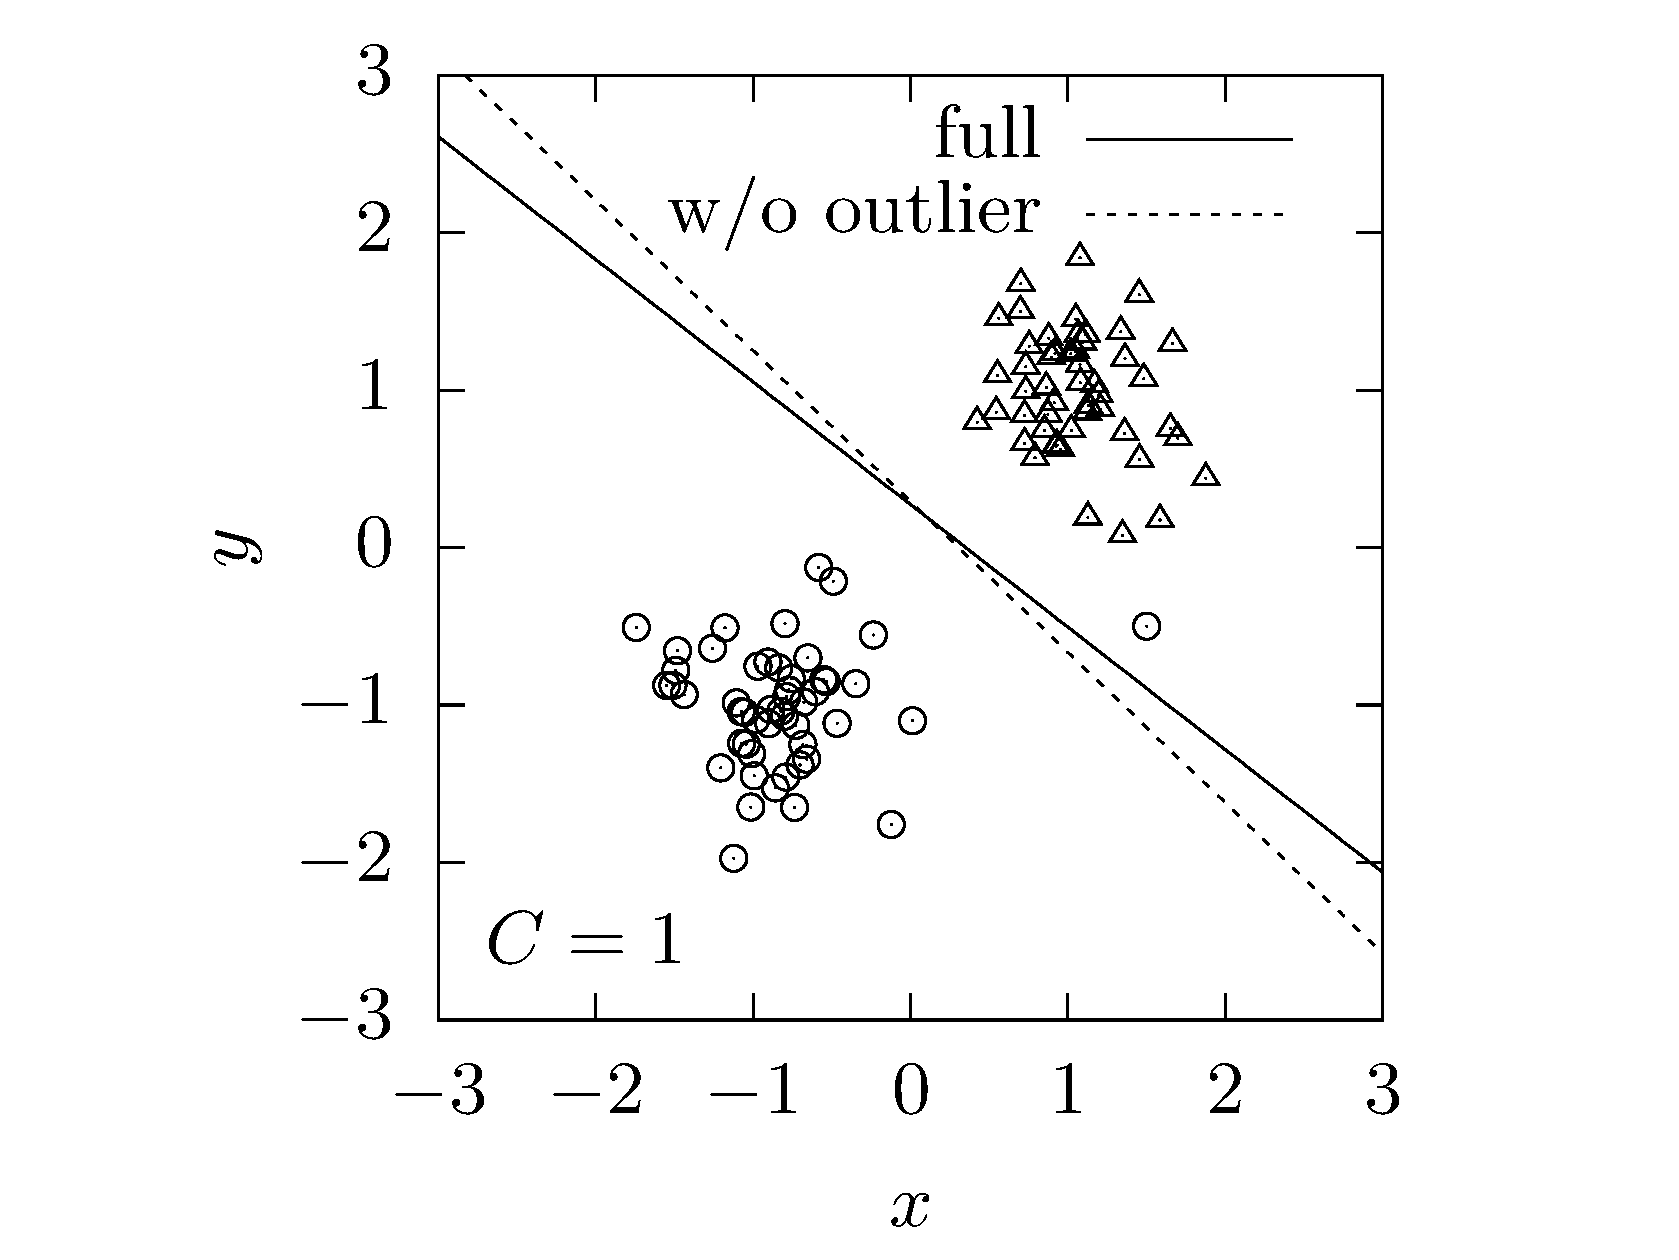
\includegraphics[scale=1.]{apdx_outliers/clf12.png}
    \end{subfigure}
    \begin{subfigure}{.49\textwidth}
        \centering
        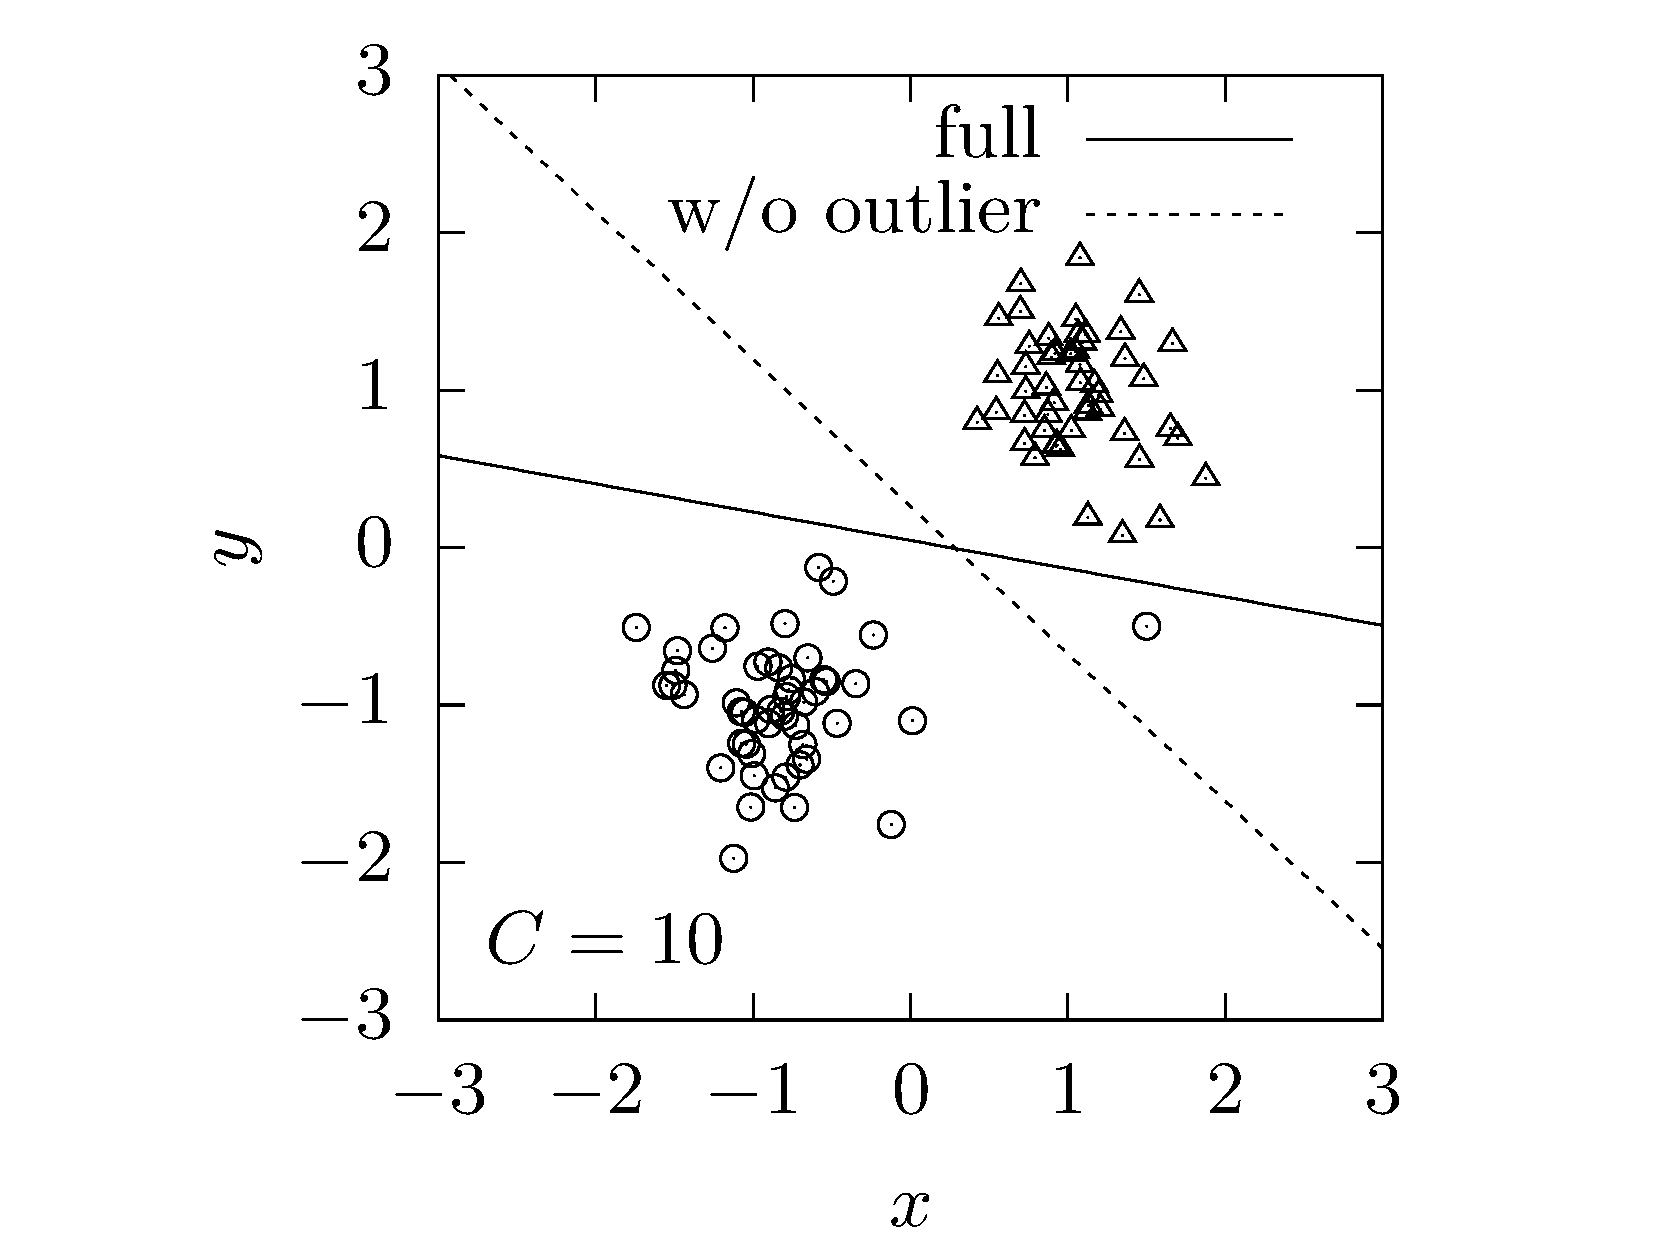
\includegraphics[scale=1.]{apdx_outliers/clf34.png}
    \end{subfigure}
    \caption{Decision boundaries of linear \glspl{svm} with different values for their respective regularization parameter $C$, trained on either the full data set (solid line) or a data set where the outlier at $(x,y)=(1.5,-0.5)$ was removed (dashed line).}
    \label{fig:apdx_svm}
\end{figure}

By their very nature, \glspl{svm} are linear classifiers for a given feature space $\vec{x}$.
The dimensionality can yet be increased by encoding higher order combinations such as $x_i^2$ or $x_i \, x_j$ in $\vec{x}$ itself, \eg{},
$$\vec x \equiv \begin{pmatrix} x_1 \\ x_2 \end{pmatrix} \; \overset{\vec\phi}{\longmapsto} \; \vec\phi \left( \vec x \right) = \begin{pmatrix} x_1 \\ x_2 \\ x_1^2 \\ x_1 \, x_2 \\ x_2^2 \end{pmatrix}.$$
The optimization problem Eq.~\eqref{eq:apdx_svm}, as well its corresponding Lagrangian dual are quadratic programming (QP) problems.
The latter QP however, only depends on inner products $\vec{x}^{\,(i)} \cdot \vec{x}^{\,(j)}$ as opposed to Eq.~\eqref{eq:apdx_svm} that depends on $\vec{x}^{\,(i)}$ itself.
This allows the application of the Mercer's theorem that guarantees the existence of a kernel function $K\! \left( \vec{x}^{\,(i)}, \vec{x}^{\,(j)} \right)$ such that 
$$\vec{x}^{\,(i)} \cdot \vec{x}^{\,(j)} \; \overset{\vec \phi}{\longmapsto} \; \vec \phi\! \left( \vec{x}^{\,(i)} \right) \cdot \vec \phi\! \left( \vec{x}^{\,(j)} \right) \equiv K\! \left( \vec{x}^{\,(i)}, \vec{x}^{\,(j)} \right),$$
if $\vec\phi$ respects the Mercer's condition.
In the present analysis we frequently use the (Gaussian) RBF kernel,
$$K\! \left( \vec{x}^{\,(i)}, \vec{x}^{\,(j)} | \gamma \right) \equiv \exp \left\{ -\gamma \left| \vec{x}^{\,(i)} - \vec{x}^{\,(j)} \right|_2^2 \right\},$$
which corresponds to a function $\vec \phi(\vec x)$ that maps $\vec x$ into an infinite-dimensional space and thus leverages the training of complex, non-linear classifier using \glspl{svm}.

For $m$ training instances and $n$ features, the complexity of training \glspl{svm} scales between $\mathcal{O}(m^2 \times n)$ and $\mathcal{O}(m^3 \times n)$, due to the inversion of the kernel matrix which makes \glspl{svm}, even if they are versatile machine learning models on small to medium sized data sets, impractical to use on large data sets.
